\documentclass[11pt]{article}

\usepackage[utf8]{inputenc}
\usepackage{hyperref}
\usepackage{graphicx}
\usepackage{csquotes}
\usepackage{amsmath}
\usepackage{url}
\makeatletter
\g@addto@macro{\UrlBreaks}{\UrlOrds}
\makeatother

\title{ Compulsory Assignment 1}
\author{
  Petter Jakub Økland\\
  \texttt{223073}
  \and
  Eivind Norling\\
  \texttt{267792}
}

\begin{document}
\maketitle

We worked together using a GitHub repository\cite{git} and delegated assignments through
a TODO file. Through Facebook we discussed the assignments and analyses as well as what
sources to add in the third assignment.

\section{The Karate Club Network}
\subsection{}
\begin{figure}
  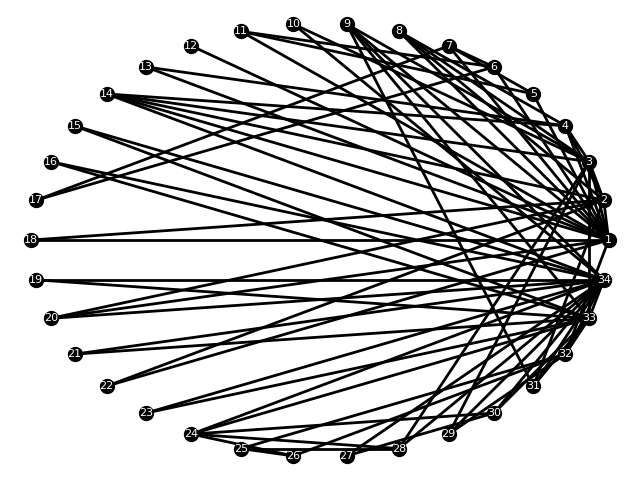
\includegraphics[width=\linewidth]{Figure_1.png}
  \caption{Graph of karate club network.}
  \label{fig:graph model}
\end{figure}

Figure \ref{fig:graph model} shows a graph of the karate club network.

\subsection{}
Zachary\cite{Zachary} analyzes the splintering of a karate club into two different organizations
over a dispute over lessen fees. He lists several reasons for formalizing this fission
process into a mathematical model, the most important perhaps being that the model is
new to anthropology.

His analysis shows how the flow of political information predicts the two opposing
factions' increasingly divergent views and strategy ultimately leading to a fission
as information flow between factions becomes increasingly hampered by a bottleneck
of information between them.

Beyond just club meetings, shared perceptions on the nature of the club communicated
in the friendship network was unable to become reconciled accross factional boundraries.
An organizational and ideological feedback relationship -- a vicious cycle-- wherein the
strategy of the factions increasingly intensified the ideological divide while threatening
the organizational basis for the network's existence itself made the fission all but
inevitable.

The form of this analysis can be applied to more than just the karate club, extending to
analysis of communication patterns in small groups in general due to the inherency of the
the feature of the minimum cut in a capacitated network in this mathematical model, which
is what made this model quite new to anthropology at the time. Whenever the existence of
a unique minimum cut in a capacitated network can be established, it will under certain
conditions (here communication of club meetings) result in a barrier to group unity which
can end up in a group fission.

\subsection{ Results of various measures in NetworkX (rounded up): }
\textbf{degree\_centrality(G)}

\begin{align*}
1: 0.48 && 2: 0.27 && 3: 0.3 && 4: 0.18 \\
5: 0.09 && 6: 0.12 && 7: 0.12 && 8: 0.12 \\
9: 0.15 && 10: 0.06 && 11: 0.09 && 12: 0.03 \\
13: 0.06 && 14: 0.15 && 15: 0.06 && 16: 0.06 \\
17: 0.06 && 18: 0.06 && 19: 0.06 && 20: 0.09 \\
21: 0.06 && 22: 0.06 && 23: 0.06 && 24: 0.15 \\
25: 0.09 && 26: 0.09 && 27: 0.06 && 28: 0.12 \\
29: 0.09 && 30: 0.12 && 31: 0.12 && 32: 0.18 \\
33: 0.36 && 34: 0.52 && &&
\end{align*}

\textbf{betweenness\_centrality(G)}

\begin{align*}
1: 0.438 && 2: 0.053 && 3: 0.14 && 4: 0.012 \\
5: 0.0006 && 6: 0.030 && 7: 0.030 && 8: 0.0 \\
9: 0.056 && 10: 0.0008 && 11: 0.0006 && 12: 0.0 \\
13: 0.0 && 14: 0.046 && 15: 0.0 && 16: 0.0 \\
17: 0.0 && 18: 0.0 && 19: 0.0 && 20: 0.032 \\
21: 0.0 && 22: 0.0 && 23: 0.0 && 24: 0.018 \\
25: 0.0022 && 26: 0.0038 && 27: 0.0 && 28: 0.022 \\
29: 0.0018 && 30: 0.0029 && 31: 0.014 && 32: 0.14 \\
33: 0.15 && 34: 0.3 && && 
\end{align*}

\textbf{closeness\_centrality(G)}

\begin{align*}
1: 0.57 &&  2: 0.49 && 3: 0.56 && 4: 0.46 \\
5: 0.38 && 6: 0.38 && 7: 0.38 && 8: 0.44 \\
9: 0.52 && 10: 0.43 && 11: 0.38 && 12: 0.37 \\
13: 0.37 && 14: 0.52 && 15: 0.37 && 16: 0.37 \\
17: 0.28 && 18: 0.38 && 19: 0.37 && 20: 0.5 \\
21: 0.37 && 22: 0.38 && 23: 0.37 && 24: 0.39 \\
25: 0.38 && 26: 0.38 && 27: 0.36 && 28: 0.46 \\
29: 0.45 && 30: 0.38 && 31: 0.46 && 32: 0.54 \\
33: 0.52 && 34: 0.55 && &&
\end{align*}

\textbf{average\_clustering(G)}

\begin{align*}0.5706384782076823\end{align*}

\textbf{connectivity.local\_edge\_connectivity(G, 1, 34)}

\begin{align*}10\end{align*}

\paragraph{Discussion} \hspace{0pt} \\
Betweenness centrality -- the most important centrality measure -- shows unsurprisingly
the two central figures with the highest score, followed by 33, 3, and 32, respectively.

32 -- along with 9, 14, and 20 -- are the only nodes with direct connections to both
central figures. Intuitively, then, we can assume they were central to information flow
between the factions.

As the local edge connectivity result shows, 10 nodes would have to be removed for
nodes 1 and 34 to become isolated from each other. It wouldn't be surprising if we
found nodes 3, 9, 14, 20, 32, and 33 among them.

\subsection{}
Figure \ref{fig:graph model2} shows another graph of the karate club network with
higlights we found important. Red nodes and edges show direct connections to node 1
in the network, blue nodes and edges show direct connections to node 34, green nodes
are those with direct connections to both nodes 1 and 34, while green edges show
connections from green nodes to nodes other than 1 and 34. Black nodes and edges are
any those without the listed criterias.

\begin{figure}
  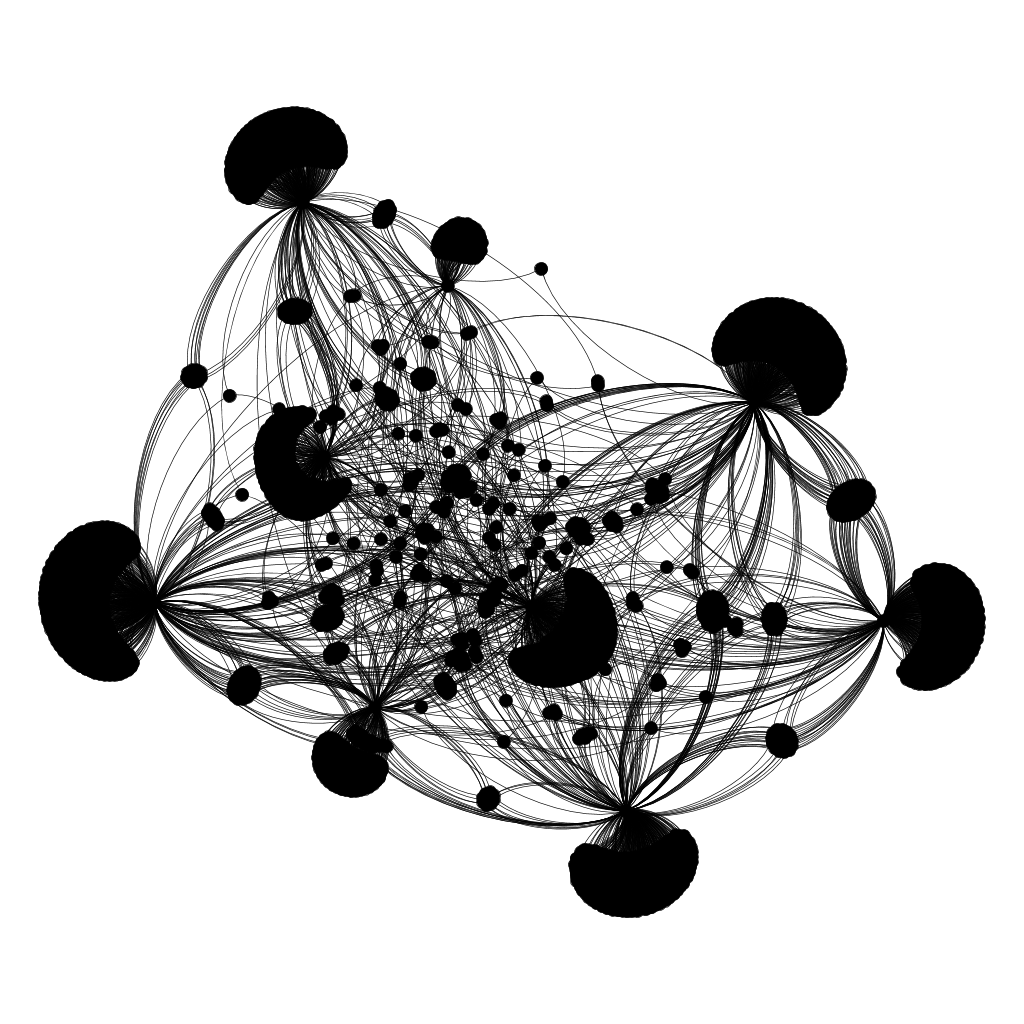
\includegraphics[width=\linewidth]{Figure_2.png}
  \caption{Graph of Karate Club network with highlights.}
  \label{fig:graph model2}
\end{figure}

\subsection{}
Discussion of analysis in light of article.

\section{Polarized blogging about climate change}
\subsection{}
\begin{figure}
  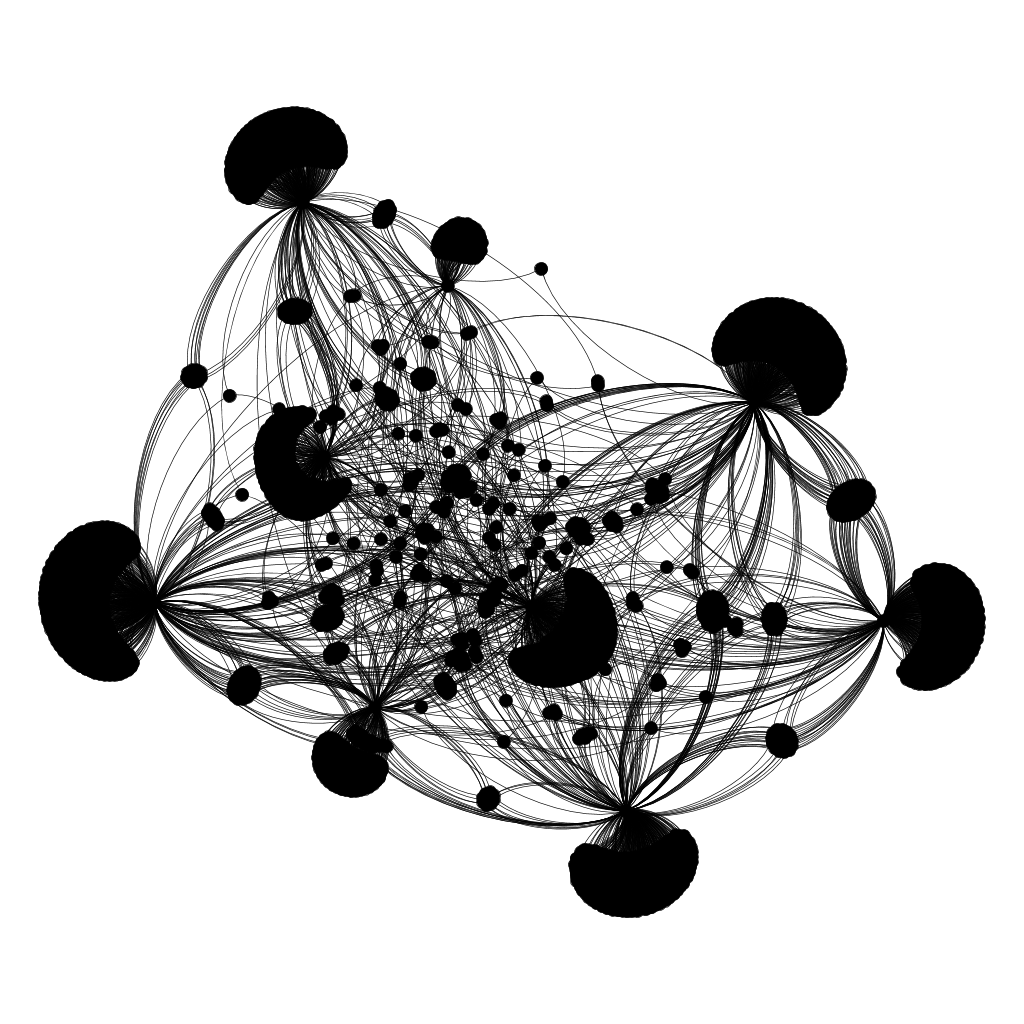
\includegraphics[width=\linewidth]{Figure_3.png}
  \caption{A graph of the network of climate blogs.}
  \label{fig:graph}
\end{figure}

Figure \ref{fig:graph} shows a graph of the network of climate blogs.

\textbf{}
\newline
\textbf{Statistics:} \hspace{0pt}

Average degree: \hfill 2.524

Network diameter: \hfill 4

Graph density (undirected): \hfill 0.001

Modularity: \hfill 0.667

Connected components: \hfill 1

Average Clustering Coefficient: \hfill 0.249

Average path length: \hfill 3.236

\subsection{}
\paragraph{https://wattsupwiththat.com/} \hspace{0pt} \\
Anthony is a former meteorologist who appears to express his position on climate
change emotively by cataloging percieved faults by those who adhere to the fact of
anthropogenic global warming in what he calles ''Climate FAIL Files''. Interestingly
he lists the following as the reason for changing his mind about climate change on
the FAQ page:

\begin{displayquote}
\textit{My questioning started due to a professional friendship that came
about with Jim Goodridge. [...] He had showed me some of his investigations into
California’s temperature and precipitation records that didn’t quite add up to some
of the claims about warming I was reading about.}
\end{displayquote}

\paragraph{https://www.desmogblog.com} \hspace{0pt} \\
The position on climate change in this blog appears to be staunchly against
the views expressed by climate deniers, aiming to catalog all disinformation
campaigns in the ''Climate Disinformation Database''. As it says on the
database page:

\begin{displayquote}
\textit{DeSmogBlog thoroughly investigates the academic and industry backgrounds of those
involved in the PR spin campaigns that are confusing the public and stalling action
on global warming.}
\end{displayquote}

\paragraph{http://joannenova.com.au/} \hspace{0pt} \\
Jo expresses her views on climate change by insinuating that scientists working on
data which confirms the reality of global warming are motivated by money and that
their data doesn't stand up to scrutiny due to things like spelling errors,
ostensible elementary mistakes in the data itself, and lack of audit and control
despite papers having to be submitted to a rigorous peer review process.

\paragraph{https://judithcurry.com/} \hspace{0pt} \\
Judith's blog presents itself on the about page as follows:

\begin{displayquote}
\textit{Climate Etc. provides a forum for climate researchers, academics and technical experts
from other fields, citizen scientists, and the interested public to engage in a
discussion on topics related to climate science and the science-policy interface.}
\end{displayquote}

There doesn't appear to be any ideological position taken and the blog's purpose
is to encourage debate around climate science.

\paragraph{http://www.climatecentral.org/} \hspace{0pt} \\
Climate Central presents themselves as follows:

\begin{displayquote}
\textit{An independent organization of leading scientists and journalists researching and
reporting the facts about our changing climate and its impact on the public.}
\end{displayquote}

They express their views on climate change as it being a reality, presents its
effects, backs it up with research and data, and discusses possible solutions to the
problem as well as what's being done and has been done so far.

\paragraph{https://insideclimatenews.org/} \hspace{0pt} \\
ICN accept the reality of climate change and seeks to act as watchdog against
governments and groups that pose a threat to the vital work needed to combat it.
They cover all news related to climate change including policies that affect it.
As it reads on their about page:

\begin{displayquote}
\textit{InsideClimate News is an independent, not\-for\-profit, non\-partisan news organization
that covers clean energy, carbon energy, nuclear energy and environmental science\-plus
the territory in between where law, policy and public opinion are shaped.}
\end{displayquote}

\paragraph{http://www.climatechangenews.com/} \hspace{0pt} \\
Very much the same as the former:

\begin{displayquote}
\textit{Climate Home News is an independent news site dedicated to bringing important climate
stories to as large an audience as possible.}
\end{displayquote}


\paragraph{http://www.realclimate.org/} \hspace{0pt} \\
RealClimate presents news about climate change in the eyes of climate scientists. It
allows comments on its posts which encourages discussion around the science of
climate change for anyone interested. Unsurprisingly they do not deny the reality of
anthropogenic global warming.  As it reads on their about page:

\begin{displayquote}
\textit{RealClimate is a commentary site on climate science by working climate scientists for
the interested public and journalists. We aim to provide a quick response to developing
stories and provide the context sometimes missing in mainstream commentary. The
discussion here is mostly restricted to scientific topics and will only rarely get
involved in any political or economic implications of the science.}
\end{displayquote}


\paragraph{https://www.skepticalscience.com/} \hspace{0pt} \\
SkepticalScience combats the misinformation by climate deniers by debunking their
claims head on and looking at what the evidence actually says. It was created by
John Cook, a cognitive scientist. As it reads on the front page:

\begin{displayquote}
\textit{Scientific skepticism is healthy. Scientists should always challenge themselves to
improve their understanding. Yet this isn't what happens with climate change denial.
Skeptics vigorously criticise any evidence that supports man-made global warming and
yet embrace any argument, op-ed, blog or study that purports to refute global warming.
This website gets skeptical about global warming skepticism. Do their arguments have
any scientific basis? What does the peer reviewed scientific literature say?}
\end{displayquote}

\subsection{}
Characterize the network

\subsection{}
Discussion in light of literature we know

\section{The psychology of social media}

\subsection{}

We chose these 10 sources to articles, videos or posts that are concerned with the
negative consequences and downsides of the usage social media and how it can affect
our mental health. We think they cover a wide variety of different aspect, research
and side effects to your mental health regarding social media.

The first source \cite{youtube1} is a YouTube video produced by BuzzFeed about Aria
Inthavong who live-streamed his entire life for 7 days, 24 hour a day onto social media.
For the duration of the livestream he had a couple thousand people watching and interacting
with the stream at all times, reacting to all his moves and judging him by his actions.
Aria himself describes this as one of his life's most mentally challenging weeks and
describes how shearing everything in your life online broke him down his mental health.

Source number two \cite{medium} is a article written by Tristan Harris. He is the
co-founder of Center for Humane Technology, previously worked for Google and has a
broad technological background. In his article, “How Technology is Hijacking Your Mind
— from a Magician and Google Design Ethicist” he talks about how technology is designed
to exploit people's mind and weaknesses.

The third source \cite{thenewatlantis} I want to bring attention to is this article
from the summer of 2010. The article is written by Roger Scruton who is a English
writer and philosopher. In his article “Hiding Behind the Screen” he talks about
human relations and how people's behavior change when they can hide behind a screen
or an avatar. He also dives into the subject of how people are seeking emotional
attention on the internet.

The fourth source \cite{youtube2} is a another YouTube video. It is published on
the youtube channel Ewafa and the video is about an interview with Sean Parker and
Chamath Palihapitiya. The video is named “Facebook is ‘Ripping Apart Society’”. The
main topics in this video is about how social media, in this case Facebook is creating
what Sean Parker is describing as a social validation feedback loop and how the big
companies are tailoring their algorithms to exploit the psychology of the human brain
on how we crave recognition and the need for “Likes” for that quick fix of a dopamine
rush. Chamath talks a lot about the same but digs a bit deeper into the phycology part.
He speaks about how humans not wants instant feedback and how we have lost our patience.

The fifth source \cite{benthamsgaze} we have chosen is a more technical article about
a phenomenon called “Like Farms”. The article does not dig much into the physiological
aspects of farming and buying likes but we still find this article relevant to the
subject and we want to look a bit deeper into this corner of the internet. “Like Farms”
are websites you can go to, to buy likes on social media. These farms usually target
sites like Facebook, Twitter and Instagram. The farming sites allow you to buy x number
of likes for your instagram post, facebook page etc. Some farms operate with hordes of
stolen, hacked or hijacked accounts controlled by bots to deliver all the likes, while
other farms are employing hundred or thousands of people from India with their own
personal army of fake accounts. We find it incredible that people are so addicted to
these imaginary points we call likes that they are willing to go to the extent of buy
them. It also amazes us that there is in fact people on this globe whos job is to create
fake social media accounts and go into paying customers media posts and pages just to
give em a dopamine rush and some fake acknowledgement.

The sixth source \cite{psychologytoday1} is from a article we found on Psychology Today
and is written in March 2016 by Martin Graff who is a professor in digital love. In his
article named “Do You Crave Facebook Likes?” he talks about his study where he looked
into what aspects of validation people seeked from social media on how it affected
their self-esteem and personality.

The seventh source \cite{psychologytoday2} is an article from Psychology Today. This
one is written by professor Mark D. Griffiths and was written in May 2018. This article
named “Addicted to Social Media?” brings up the topic of what can be done to reduce the
excessive use of social media.

The eight source \cite{youtube3} is a YouTube video that have gone viral. The video was
posted August 8, 2016 on the YouTube channel “Freedom in Thought” with the title “WHY I
QUIT SOCIAL MEDIA FOR A YEAR AND WHAT I LEARNED”. In his video he describe that he quit
social media because he was compulsively checking his phone for social media updates. He
describes how he before replaced a lot of the things he used to enjoy in life and tried
to kill both time and socially awkward situations by hiding behind his phone. The first
half of the video he describes how the social media machinery is wired to abuse
weaknesses in our brain and constructed to consume as much attention from each user as
possible to keep them on the platforms for as long as possible.

In the second half of the video he talks about how quitting social media helped him stay
focused for extended amounts of time, relieved stress and created a distraction free
environment so he could focus his energy into other things he enjoy.

The ninth source \cite{lifehack} we want to bring to attention is this blog-post posted
on Lifehack by Heather Poole. In her post she talks about how we build these huge
networks of “fake” friends over the years while using Facebook. Everytime we meet a new
person we add each other on social media platforms even though we never see or speak to
that person again. We have friends we knew from middle school that we have not seen in
8 years but still like and comment on each others photos. We only see the sides of life
the person want to shear with the world. On social media everyone paints their own
version of themself and for most people that is the happy side where everything is
glitter and gold. She suggest to filter out and delete the friends you haven’t had a
offline conversation to do with in the last year. Heather claims this is a good way to
keep a healthy relationship to your social media friends.

The tenth and final source \cite{economist} is a article from The Economist named “How
heavy use of social media is linked to mental illness” and the article is talking about
exactly what the title implies. The article refers a graph showcasing the different
positive and negative aspects of four different social media sites. The sites are
Instagram, Snapchat, Facebook and Twitter and it uses color to describe how positive
or negative the different aspects are affecting people from 14 to 24 years-old. They
have different factors like sleep, bullying and body image.

\paragraph{Summary} \hspace{0pt} \\
To summarize all the the ten sources above, they all are the result of the big
corporations created the social medias trying to keep you on their site for as long as
possible. Apps where you maintain fake relationships and present your fake life to fake
friends.  We get addicted to these interactions and crave the need for instant
recognition. Some are even willing to pay for it, for a quick fix of dopamine and
bragging rights. This constant social validation feedback loops are what is fuling the
social media machinergy. You stay at the big corporations applications, they earn more
money from your data habits and by drowning you with ads. Then they revenu earned goes
back into research on how to manipulate you even more and keep you on their platforms.
Every time you refresh a page, you are awarded with new content and information. This
is food for your brain and our brains love to learn. This is triggering our dopamine
receptors, and as we continue to repeat this loop we keep strengthening this loop, and
addiction.

The main thing we can see from all these sources is that this is simply not good for us.
If we look at Arias video from BuzzFeed we can see that concentrated amounts of social
media interaction can break down a human emotialy in pretty fast. While excessive and
compulsive usage of social media has many downsides, Freedom in Thought’s video shows
us that completely abandoning social media can both be a positive and healing experience
that can make you more happy.

\pagebreak
\bibliography{references.bib}
\bibliographystyle{ieeetr}

\end{document}
